\chapter{Die Kinect}
\label{ch:kinect}
\Autor{Johannes Böhler}\\\\
Die drei Haupt-Hardware-Komponenten der Kinect sind ein Infrarotprojektor, eine RGB-Kamera sowie eine Infrarotkamera.\\
\begin{figure}[!ht]
  \centering
  \makebox[\textwidth]{%
   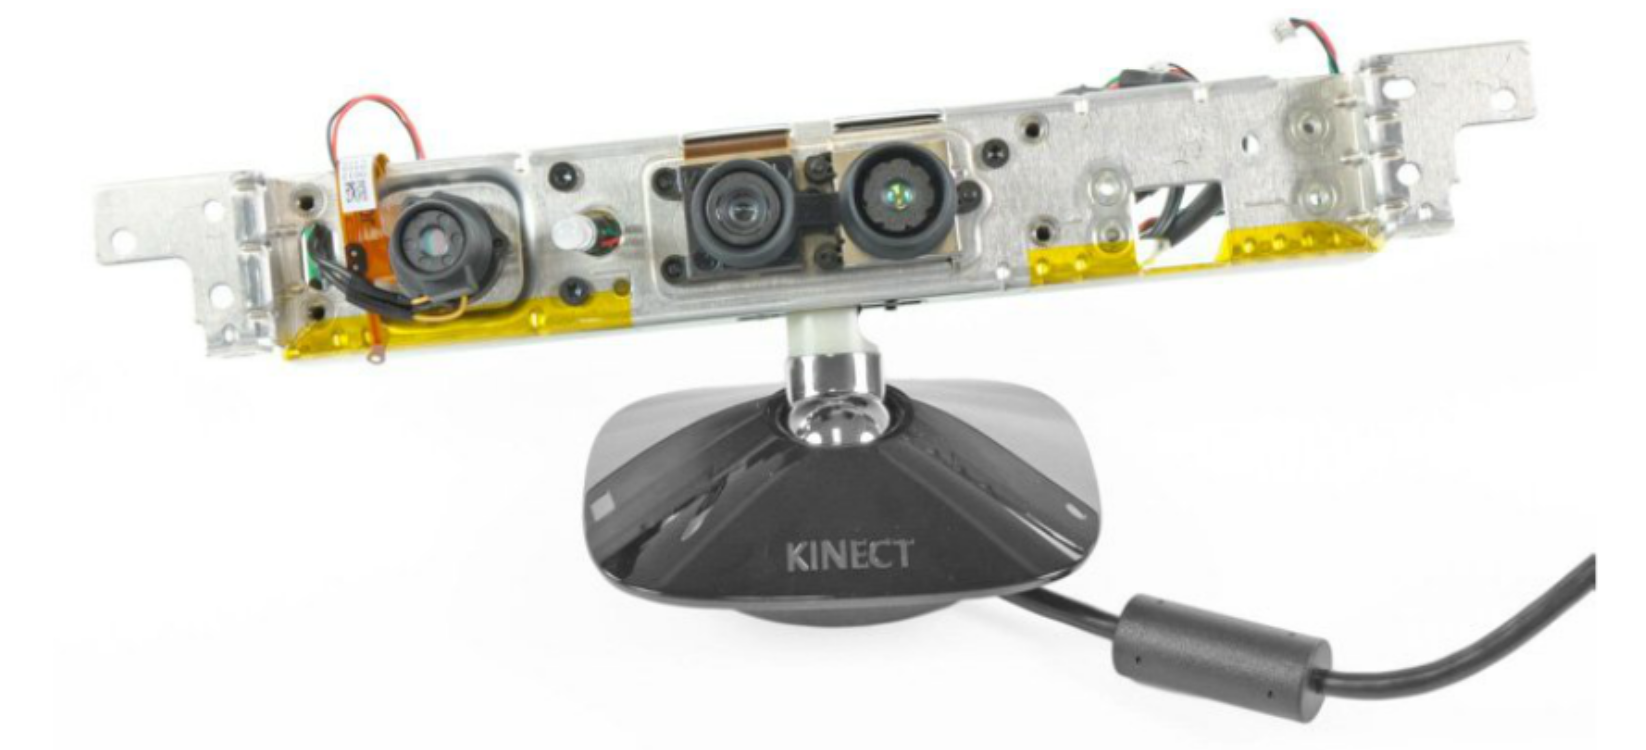
\includegraphics[height=5cm]{Res/Kinect_Components.png}
  }
   \caption{\emph {Links:} Infrarotprojektor \emph {Mitte:}: RGB-Kamera  \emph {Rechts:}: Infrarotkamera }
\end{figure}
Die Kombination aus Infrarotstrahler und Infrarotkamera ermöglicht die Gewinnung von Tiefeninformationen aus der Umgebung. Im Gegensatz zu gewöhnlichen Kameras, welche einem Pixel Farbinformation (z.B.  über RGB-Farbkanäle) zuordnen, wird dem Pixel mit Hilfe der Infrarot Kamera eine Entfernung zugeordnet.

\begin{figure}
\centering
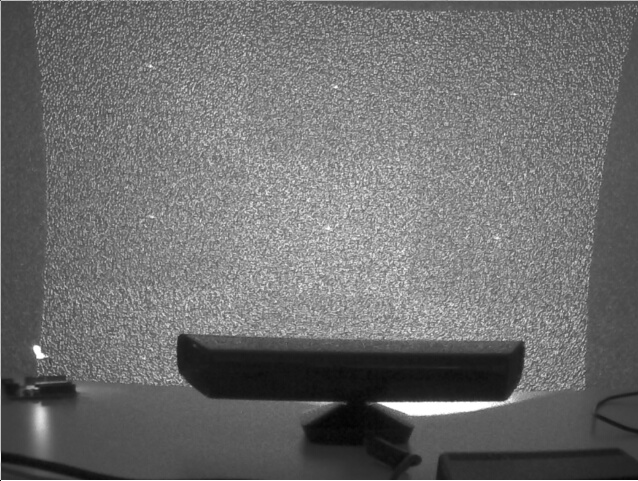
\includegraphics[width=0.5\linewidth]{./Res/Kinect_9Points}
\caption{Vom Infrarotprojektor ausgestrahltes strukturiertes Licht}
\label{fig:Kinect_9Points}
\end{figure}

%\begin{wrapfigure}{r}{0.4\textwidth}
%  \vspace{-20pt}
%  \begin{center}
%        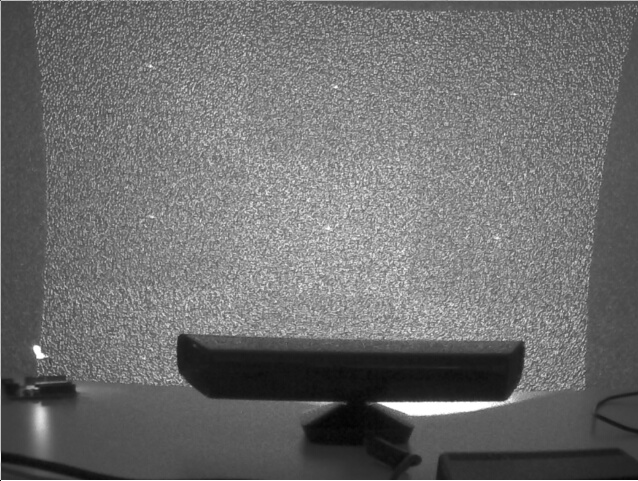
\includegraphics[height=5cm]{Res/Kinect_9Points.png}
%  \end{center}
%  \vspace{-20pt}
%  \caption{Vom Infrarotprojektor ausgestrahltes strukturiertes Licht } %
 % \vspace{-10pt}
%\end{wrapfigure}

Diese ergibt sich aus der Art und Weise wie der Infrarotstrahl von dem durch den Pixel repräsentierten Bereich eines Objektes reflektiert wird.\\

Die Tiefenbilder welche man von der Infrarotkamera erhält, sehen aus wie komplett verrauschte Graustufenbilder. Hierbei steht jeder Grau Wert eines Pixels für die entsprechende Entfernung des korrespondierenden Objektausschnittes zur Kinect.\\
Hohe Grauwerte (helle Pixel) repräsentieren nahe Objekte, während niedrige Grauwerte (dunkle Pixel) weiter entfernte Objekte beschreiben. In einem Tiefenbild ist die gesamte Information über die Entfernung der im Bildausschnitt erfassten Objekte zur Kinect enthalten.\\\\
Wird die Tiefeninformation dazu genutzt um die Pixel im dreidimensionalen Raum anzuordnen, erhält man eine Punktwolke. Die in der 2d
-Betrachtung benachbarte Pixel müssen in der 3d-Repräsentation nicht miteinander verbunden sein, da die Z-Koordinate unterschiedliche Werte aufweisen kann.
\subsection{Funktionale Komponenten}
\subsubsection{Infrarotprojektor}
Der Infrarotprojektor emittiert elektromagnetische Strahlen, deren Wellenlänge (830nm) außerhalb des für den Menschen sichtbaren Bereichs (380nm-780nm) liegt .
Der Projektor strahlt zur Tiefenbestimmung ein Gitter von Infrarotpunkten (strukturiertes Licht) auf die Objekte in seiner Umgebung ab. 
Zur Generierung dieses Musters wird ein besonderes Verfahren implementiert.
Normalerweise produzieren Filter, die diese Art von Muster generieren einen sehr hellen Punkt in der Mitte des Bildes, welcher die Leistungsfähigkeit des Infrarotprojektors limitiert. Durch das hier verwendete Verfahren entstehen statt einem einzigen sehr hellen, neun helle Punkte, welche durch unvollständige Lichtfilterung zur Mustererstellung entstehen. Das hier eingesetzte Verfahren produziert weniger starke Artefakte und ermöglicht die Verwendung einer leistungsfähigeren Diode. Dies führt zu einer höheren Genauigkeit der Abstandsauflösung und zu einer größeren Reichweite im Bezug auf die Umgebung in welcher die Entfernungsmessung durchgeführt wird. Die Reichweite des Infrarotprojektors ist dennoch eingeschränkt, da zu hohe Intensitäten der Infrarotstrahlen Augenschäden verursachen könnten.
\begin{figure}
\centering
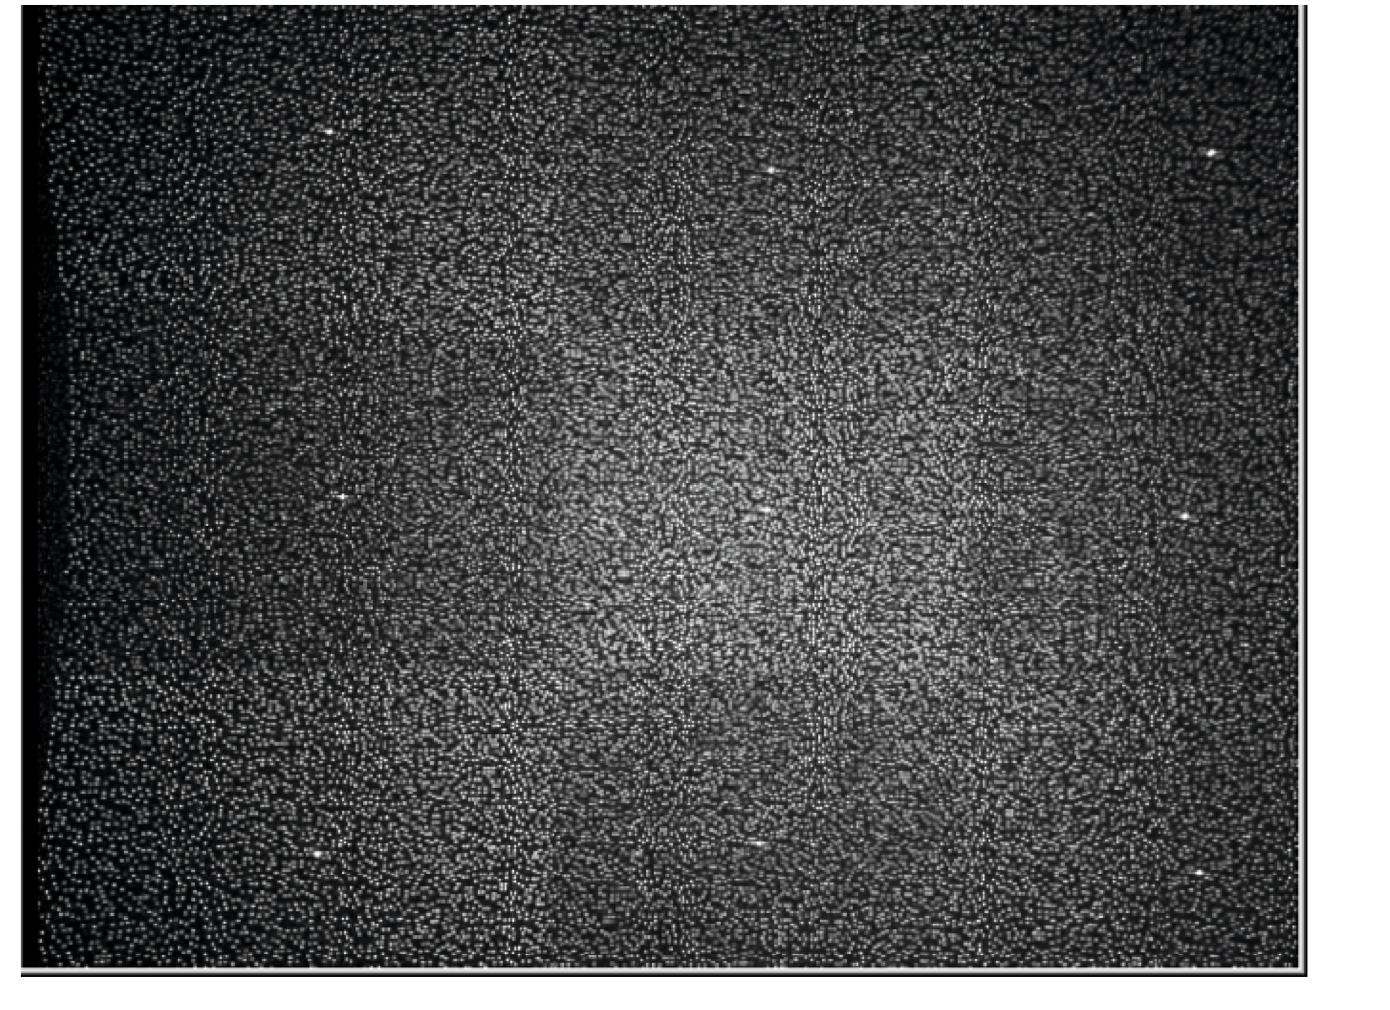
\includegraphics[width=0.5\linewidth]{./Res/9_Dots}
\caption{Gernerierung des Infrarot Random-Patterns mit Hilfe von 9 Bereichen}
\label{fig:9_Dots}
\end{figure}
\FloatBarrier
%\begin{wrapfigure}{r}{0.5\textwidth}
%  \vspace{-20pt}
%  \begin{center}
%        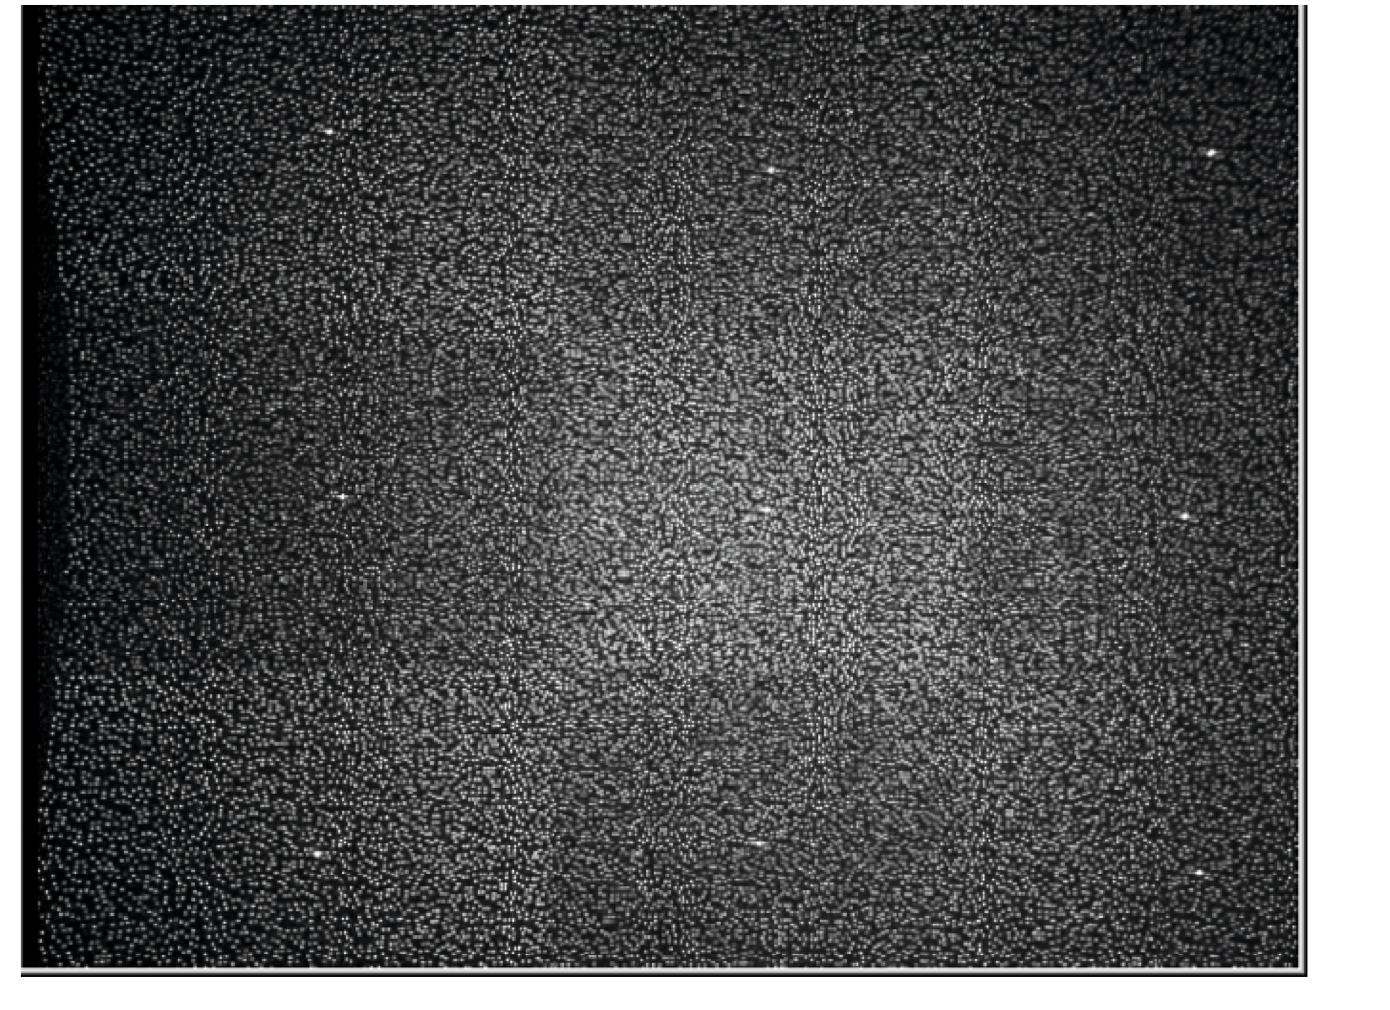
\includegraphics[height=6cm]{Res/9_Dots.png}
%  \end{center}
%  \vspace{-20pt}
%  \caption{Gernerierung des Infrarot Random-Patterns mit Hilfe von 9 Bereichen }
%  \vspace{-10pt}
%\end{wrapfigure}

\subsubsection{Infrarotkamera}
Die Infrarotkamera nimmt Bilder mit einer nativen Auflösung von 1280x1024 Pixeln, bei einer Bildwiederholrate von 30 Hz auf. Weitergeleitet werden allerdings nur Bilder mit einer Auflösung von 640x480 Pixeln, da der USB Datenbus eine Limitierung bezüglich der Datenübertragungsrate darstellt. Das Blickfeld der Infrarotkamera beträgt in der Horizontalen 58 °, in der Vertikalen 45 °. Damit die Mustererkennung funktioniert, ist ein Mindestabstand von 0,8 Metern erforderlich. \\
 \begin{figure}[!ht]
 	\begin{center}
 		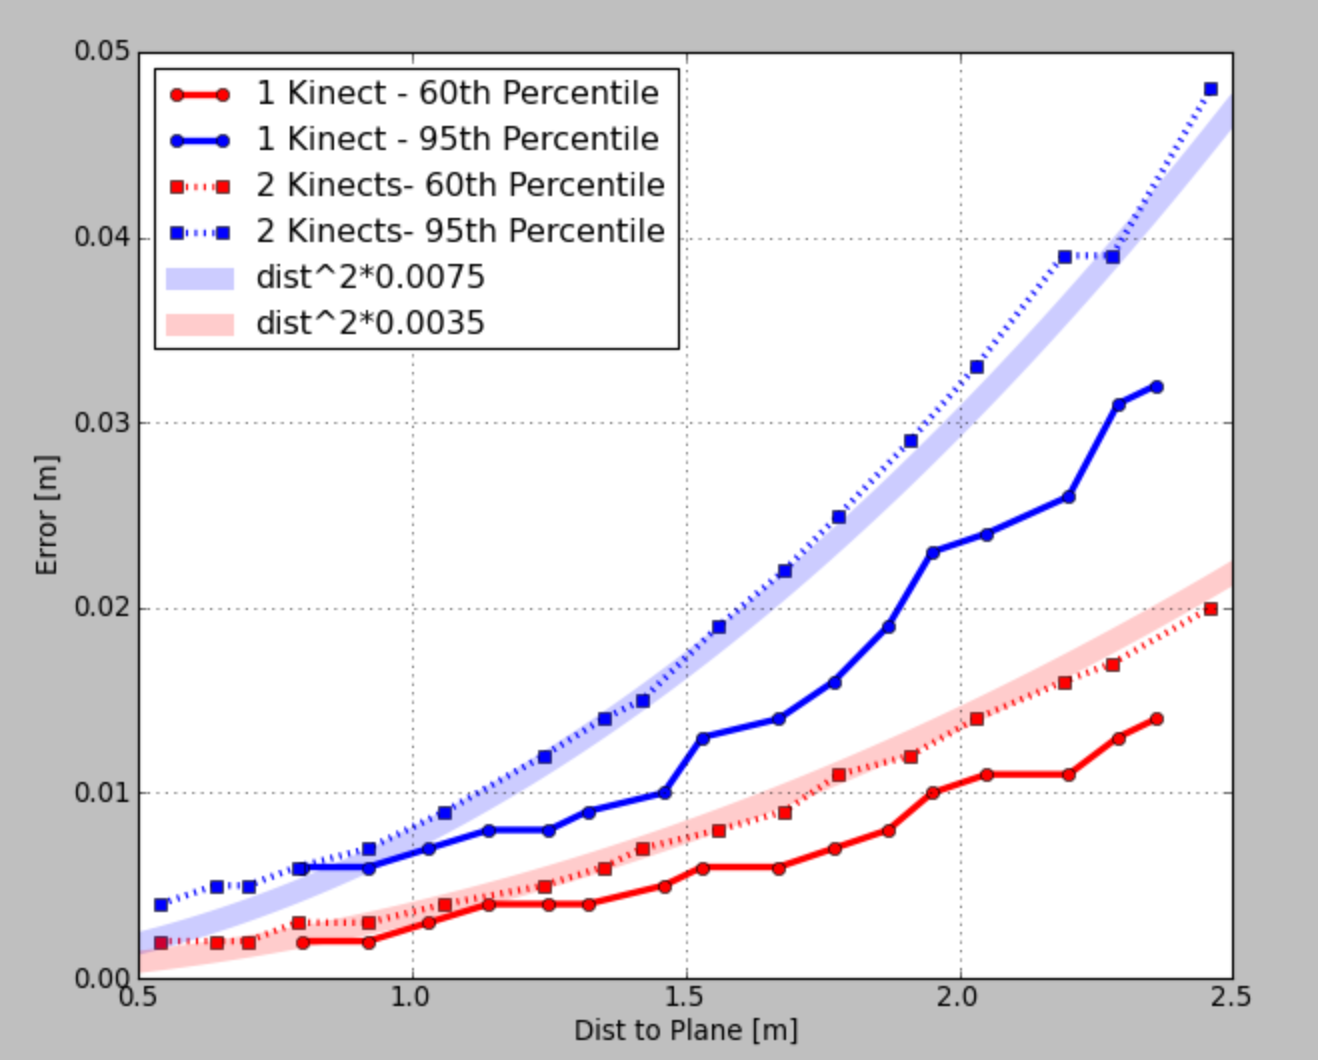
\includegraphics[width=0.65\textwidth]{./Res/Res_to_Dist}
 	\end{center}
 	\caption{Fehlerbehaftung  der Tiefeninformation in Abhängigkeit von der Objektentfernung}
 	\label{fig:Res_to_Dist}
 \end{figure}
 
 Ab einer Entfernung von 3,5 Metern wird die Intensität der reflektierten Strahlen zu gering um Tiefeninformationen mit ausreichender Aussagekraft und Präzision zu erhalten.
Bei einem optimalen Abstand von 2 Metern zum Objekt beträgt die Auflösung 
in der XY-Ebene 3 mm, in der Z-Ebene 1 cm.





Die Quantisierungsauflösung liegt bei $2^ {11}$ (2048) Bit.
Es muss sichergestellt werden, dass die Infrarotkamera nur die erwünschte elektromagnetische Strahlung im 830 nm Bereich aufnimmt und nicht von Strahlen anderer Wellenlänge gestört wird. Dies wird durch einen Filter, welcher auf dem Infrarot-Kamera-Objektiv angebracht ist realisiert.
Trotz Verwendung des Filters sollte die Kinect in abgedunkelten Innenräumen verwendet werden, da Sonnenlicht auch elektromagnetische Wellen im Infrarotbereich enthält.

\subsubsection{RGB Kamera}
Die RGB Kamera nimmt bei einer Wiederholrate von 30 Hz ebenfalls mit einer Auflösung von 640x480 Pixeln auf, könnte jedoch auch mit einer Auflösung von 1280x1024 Pixeln bei einer reduzierten Wiederholrate von 15 Bildern pro Sekunde angesteuert werden.
Die Quantisierungsauflösung der Kamera liegt bei $2^{8}$ (256) Bit. 
\subsubsection{Mikrofon Array}
Die Kinect beinhaltet vier Mikrofone, welche verteilt verbaut sind. Sie dienen sowohl der Erfassung von Ton, als auch der Lokalisierung und Unterscheidung von Soundquellen. Hierdurch ist es möglich, unterschiedliche Stimmen mehrerer Spieler eindeutig ihren jeweiligen Avataren zuzuweisen. Jedes der Mikrophone tastet mit einer Quantisierungsauflösung von $2^{16}$ (65536) Bit und einer Abtastrate von 16 KHz ab.
\subsection{Tiefenberechnung}
Die Berechnung der Objektentfernungen (Tiefenwerte) innerhalb der Kinect erfolgt durch Aussendung von strukturiertem Licht durch die Projektionseinheit (siehe Abschnitt \emph{Infrarotkamera}) und durch Weiterverarbeitung der durch die Infrarotkamera empfangen reflektierten Strahlen. Das Muster für das strukturierte Licht wird mit Hilfe eines Diffusors (eine Lochplatte mit fest definiertem Muster) erzeugt.\\
Das Prinzip des strukturierten Lichts ist an ein Verfahren angelehnt, welches sich Streifenprojektion nennt und in dieser Anwendung modifiziert wurde, um die Erfassung von beweglichen Objekten zu ermöglichen. Anstatt von Lichtstreifen wird eine Punktematrix verwendet, welche zufällig und fest definiert ist. Die Infrarotkamera sowie der Projektor müssen sich hierzu in einem vordefinierten, gleich großen Abstand zueinander befinden.
Die Umgebungsreflektionen der projizierten Punktematrix werden von der Infrarotkamera erfasst.
Um aus diesem Gitter von reflektierten Infrarotpunkten Tiefeninformation zu extrahieren, wird das Verfahren der aktiven Stereotriangulation verwendet.\\\\
Die Triangulation ist ein Verfahren zur optischen Abstandsmessung, welches sich hierzu trigonometrischer Funktionen innerhalb von aufgespannten Dreiecken bedient. 
Es wird allgemein zwischen aktiver und passiver Triangulation unterschieden.
Aktive Triangulation bedingt mindestens eine strukturierte Lichtquelle zur Abstandsberechnung, während dies bei passiver Triangulation nicht der Fall ist.\\

Da der Infrarotprojektor ein statisches Pseudozufallsmuster emittiert, ist dieser als strukturierte Lichtquelle einzuordnen.
Stereotriangulation bedeutet dass zwei unterschiedliche Bildquellen benötigt werden um die Tiefe jedes Pixels eines Bildausschnittes berechnen zu können.
Eine der zwei Bildquellen ist der Diffusor (das „Lochmuster“), welcher die vom Projektor emittierten Strahlen statisch definiert. Die andere Bildquelle ist die Infrarotkamera.
Das "Bild" (die Lochmaske) des Projektors ist immer identisch und statisch. Das Bild der Infrarotkamera hingegen variiert je nach Umgebung. Diese beiden Bilder sind die Grundlage für die trigonometrischen Operationen zur Berechnung der Tiefeninformationen.

\begin{figure}[!ht]
  \centering
  \makebox[\textwidth]{%
    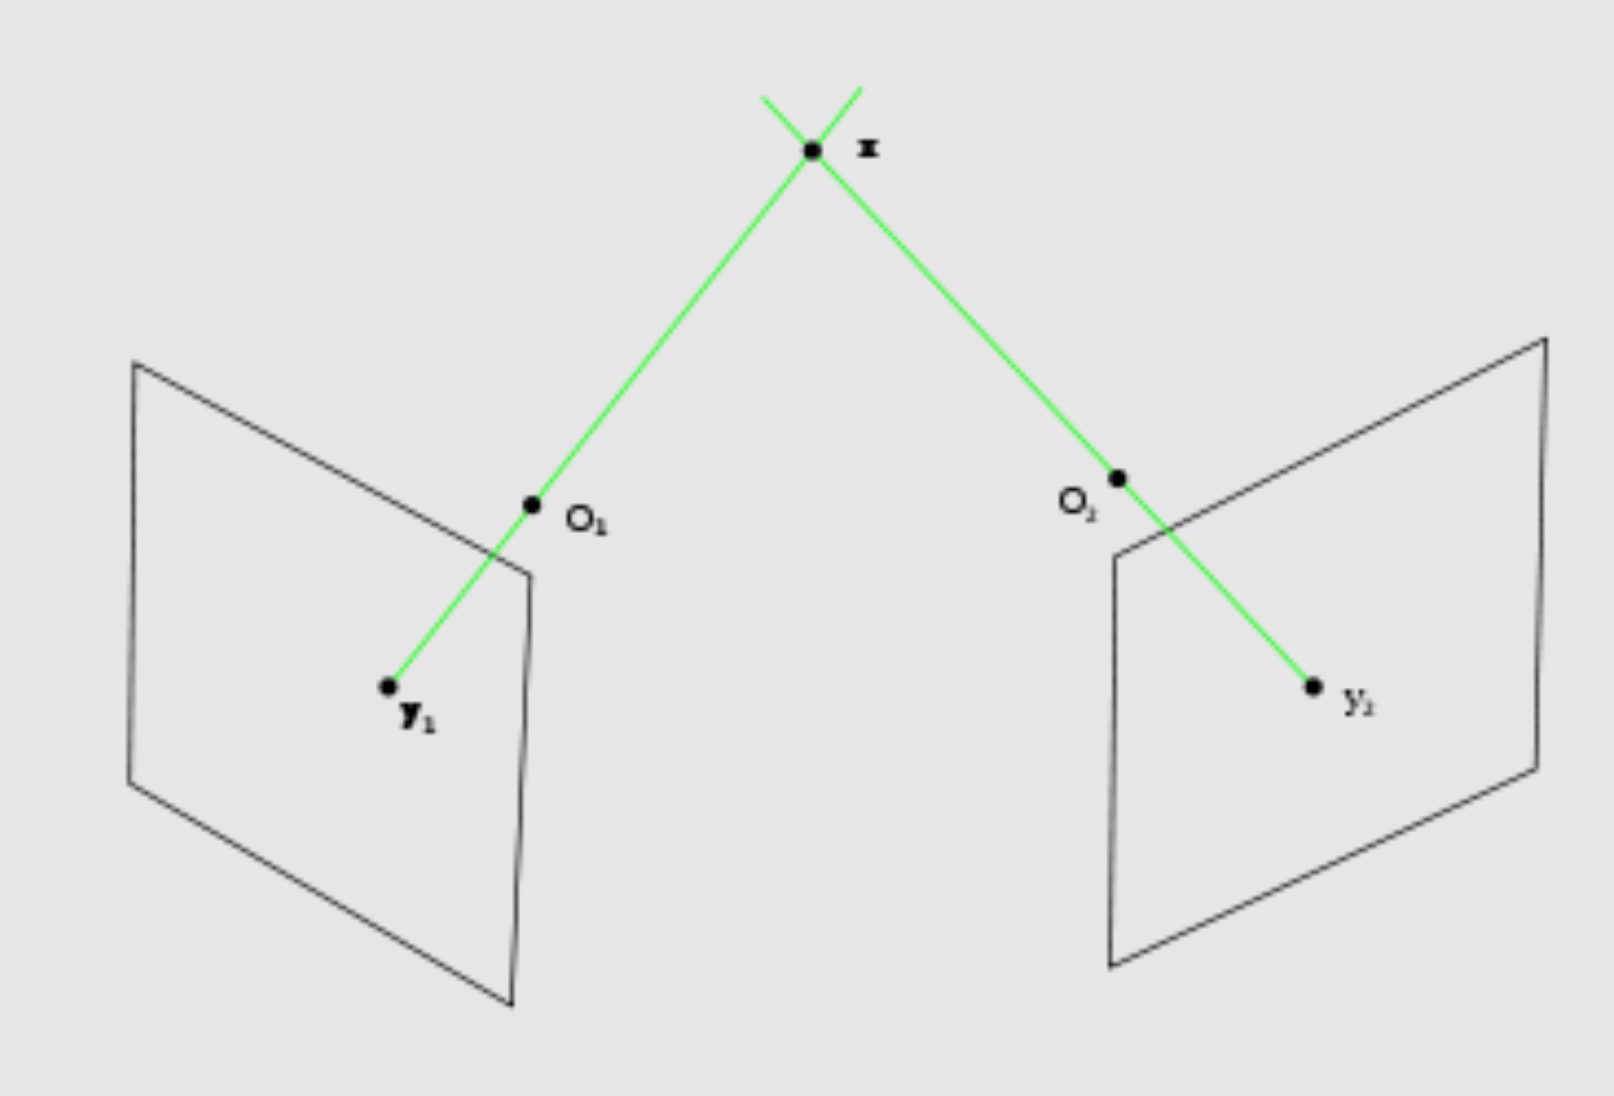
\includegraphics[height=6cm]{Res/Triangulation.png}
  }
   \caption{ aktive Stereotriangulation }
\end{figure}
Zur Gewinnung der Tiefeninformation wird die horizontale Differenz des Punktes Y1 des von der Infrarotkamera aufgenommenen Bildes zum korrespondierenden Punkt Y2 des virtuellen, statischen Referenzbildes des Projektors berechnet. Aus dieser Differenz lässt sich die Tiefe des betreffenden Pixels durch aufstellen der beiden Projektionslinien und Schnittpunktbestimmung derselben berechnen. \\
Der Grund weshalb die Pixel der statischen „Schablone“ im Projektor zufällig angeordnet sind, liegt darin, dass die unterschiedlichen lokalen Nachbarschaftsbedingungen die Pixelzuordnung zwischen dem statischen und dem dynamisch veränderten Bild erleichtern.


\subsection{Das Schattenproblem}

Aufgrund der Entfernung der verbauten RGB-Kamera zur Infrarotkamera, weisen die Bilder beider Kameras einen kleinen Versatz auf.
Schatten im Tiefenbild entstehen aufgrund der Entfernung des Infrarotprojektors zur Infrarotkamera.


\begin{figure}[!ht]
  \centering
  \makebox[\textwidth]{%
    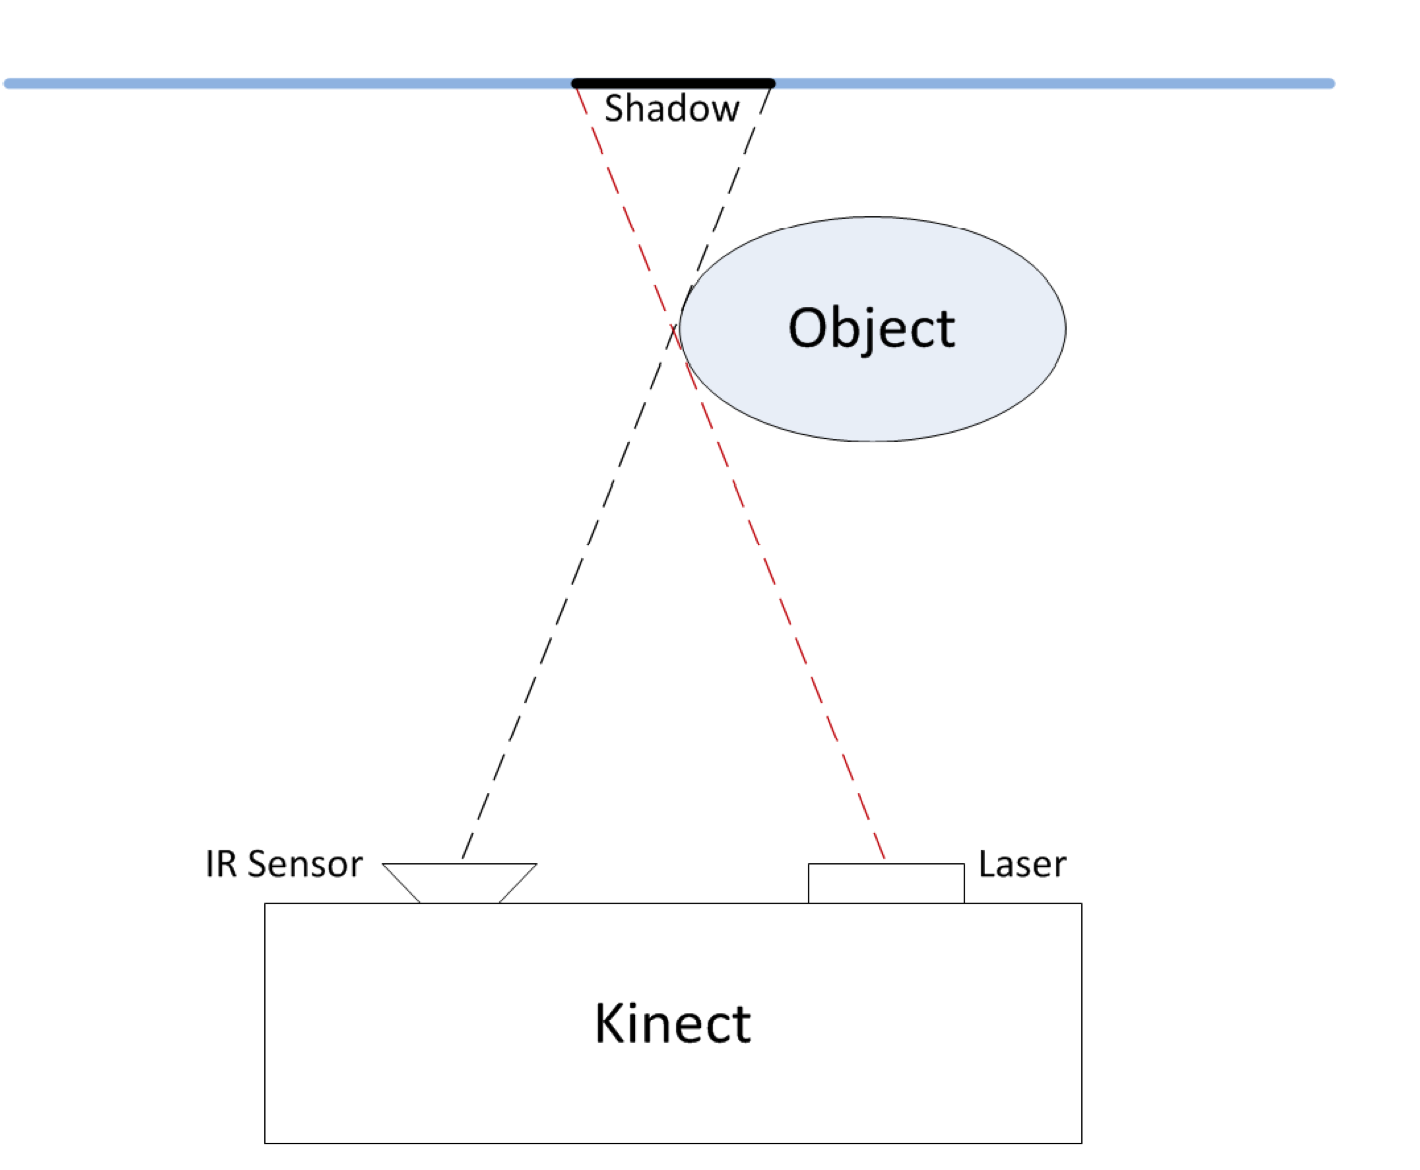
\includegraphics[height=6cm]{Res/Schatten_Strahl.png}
  }
   \caption{Blockierte Infrarotstrahlen }
\end{figure}
Der Schatten im Muster macht es für den Sensor unmöglich die Tiefe festzustellen. Die Pixel in diesen Bereichen werden stattdessen auf den Wert 0 gesetzt.
Das Objekt blockiert die Strahlen des Lasers. Da für die Tiefenberechnung das vom Infrarotprojektor emittierte Musters benötigt wird, ist es für die Kinect unmöglich die Distanz in Bereichen zu berechnen, welche außerhalb der Erreichbarkeit des Infrarot-Strahlenmusters liegen. 
\begin{figure}[!ht]
  \centering
  \makebox[\textwidth]{%
   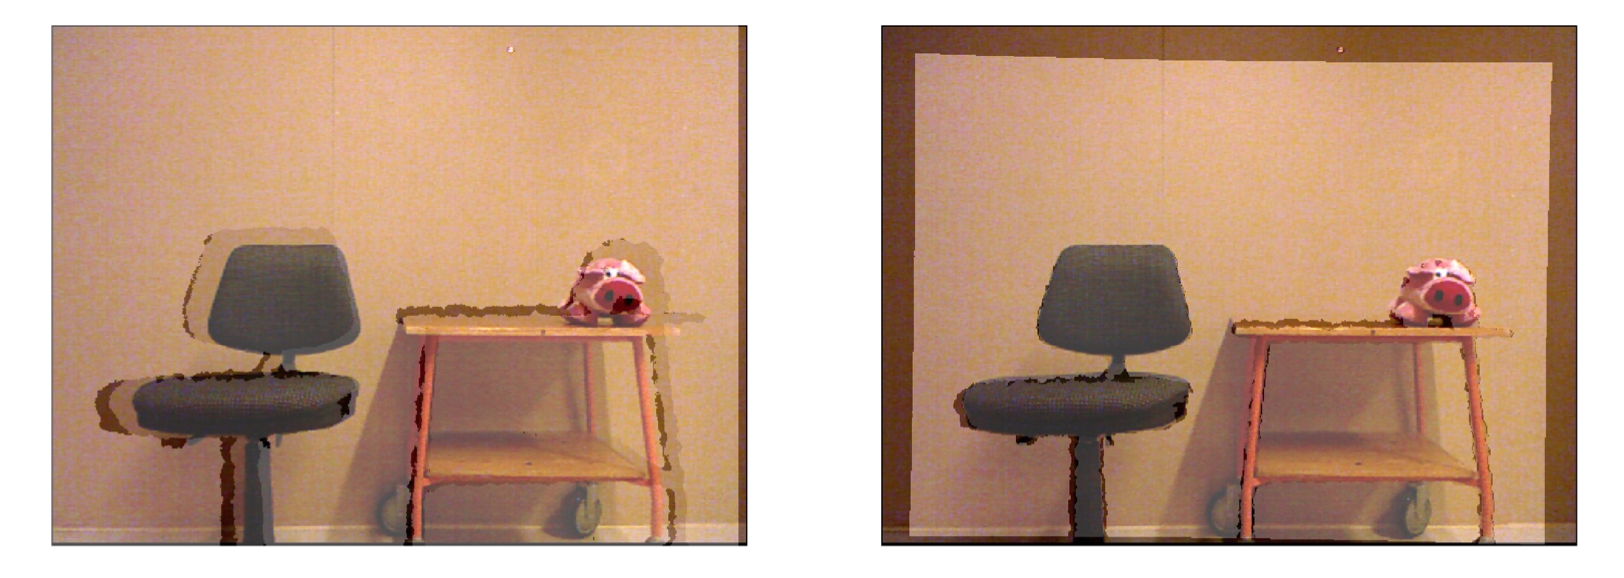
\includegraphics[height=5cm]{Res/Schatten.png}
  }
   \caption{Da der Infrarot Sensor links des Projektors positioniert ist, treten die Schatten auch linksseitig der Objekte auf.  }
\end{figure}